\documentclass[10pt,twocolumn,twoside,slovak,a4paper]{article}

\usepackage[slovak]{babel}
\usepackage[T1]{fontenc}
\usepackage[IL2]{fontenc} % lepšia sadzba písmena Ľ než v T1
\usepackage[utf8]{inputenc}
\usepackage{graphicx}
\usepackage{url} % príkaz \url na formátovanie URL
\usepackage{hyperref} % odkazy v texte budú aktívne (pri niektorých triedach dokumentov spôsobuje posun textu)
\usepackage{graphicx}
\usepackage{cite}
\usepackage{todonotes}
\usepackage{rotating}
\usepackage{times}

\pagestyle{headings}

\title{Uživateľské údaje zbierané odporúčacími systémami\thanks{Semestrálny projekt v predmete Metódy inžinierskej práce, ak. rok 2024/25, vedenie: Richard Marko}} % meno a priezvisko vyučujúceho na cvičeniach

\author{Dmytro Bykov\\[2pt]
	{\small Slovenská technická univerzita v Bratislave}\\
	{\small Fakulta informatiky a informačných technológií}\\
	{\small \texttt{xbykov@stuba.sk}}
	}

\date{\small 3. október 2024} % upravte



\begin{document}

\maketitle

\begin{abstract}
V dôsledku rozvoja umelej inteligencie, internetové biznisy začali implementovať do svojich systémov takzvané "Odporúčacie systémy". S ich pomocou môže mechanizmus automaticky ukazovať jednotlivým použivateľom odlišný obsah na internet stránkach v závislosti od ich preferencii. Aby vedeli fungovať, musia zbierať data použivateľov čo stránky navštevujú. Táto práca je zamerianá na vysvetlenie rozdielov v práci jednotlivých odporúčacich systémov. Na začiatok je potrebné pochopiť, čo spája všetky odporúčacie systémy. Následne je dôležité uvedomiť si, aké rôzne systémy existujú a v čom sú ich rozdiely. Nakoniec je užitočné analyzovať, aké môžu nastať problémy pri používaní jednotlivých odporúčacích systémov.
\end{abstract}

\begin{sidewaysfigure}
\centering
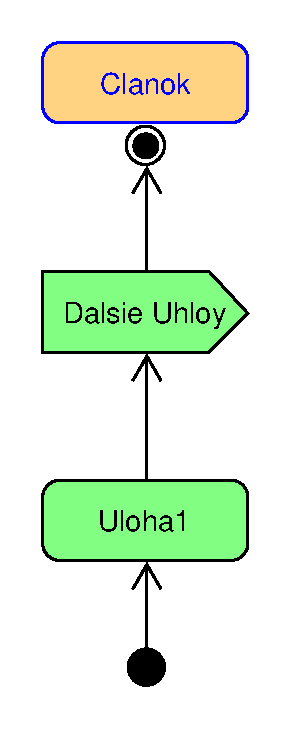
\includegraphics[height =2in,width=1in]{progres_mip.pdf}
\end{sidewaysfigure}
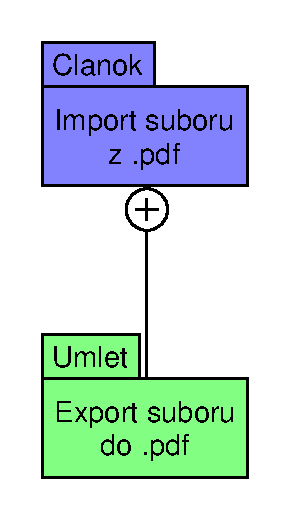
\includegraphics[height =2in,width=1in]{diagram_2.pdf}

\section{Úvod}

Veľkým pokrokom v rozvoji umelej inteligencie boli a zostávajú odporúčacie systémy. Sú to systémy, ktoré dokážu predpovedať, aký obsah by používateľa mohol zaujímať. Dnes sa používaju vo väčšine on-line biznisov. Napriek natoľko rozšírenému používaniu týchto systémov, princíp ich práce ostáva pre používateľov neviditeľný. Veľkú neistotu vyvoláva otázka, aké používateľské údaje sú systémami zbierané. Keďže odporúčacie systémy často pracujú na základe osobných informácii o použivateľovi, nie vždy je možné do konca predvídať, aké informácie budú zapísané v databázach. Podľa prieskumu spoločnosti Ping Identity z roku 2024 až 97\% z opýtaných majú obavy ohľadom toho, že ich údaje sú dostupné v internet priestore\cite{Ping:Fear}. Preto je potrebné pochopiť, na základe akých informácii odporúčacie systémy pracujú. 


\begin{figure*}
\centering
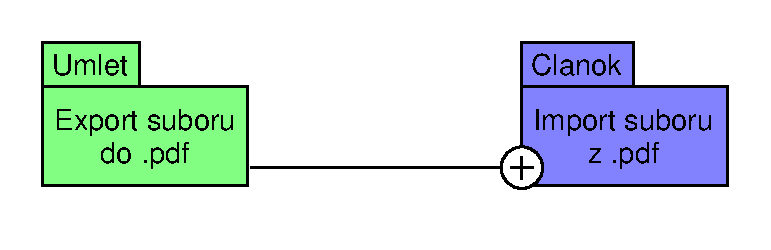
\includegraphics[height =1in,width=\textwidth]{diagram_3.pdf}
\end{figure*}


\section{Rôzne typy odporúčacích systémov}

\section{Hlavné rozdiely medzi rôznými odporúčacími systémami}

\section{Dôvody pre obavy o svoje data}

\bibliography{literatura}
\bibliographystyle{abbrv} % prípadne alpha, abbrv alebo hociktorý iný
\end{document}